% SPDX-License-Identifier: CC-BY-4.0
\documentclass{article}
\usepackage[margin=1in]{geometry}
\usepackage{graphicx} 
\usepackage[colorlinks=true, urlcolor=blue, linkcolor=red]{hyperref}

\begin{document}
\author{David Meeker}
\title{Bonded NdFeB Magnet Properties}
\maketitle

Bonded NdFeB properties defined in FEMM are meant to be representative of typical examples rather than strictly based on the products from one vendor. 

Since bonded magnets consist of permanent magnet powder with a polymer binder, the electrical conductivity is very low.  A typical value of electrical conductivity is 0.01 MS/m.

Low energy product bonded magnets have a relative permeability closer to 1.  As the energy product increases, the relative permeability of the material also increases.  By regressing data provided in manufacturer's literature, a reasonable model for the dependence of relative permeability on energy product is:

\[\mu_r = 1.06 + 0.02 \left( \frac{bhmax}{\mbox{MGOe}} \right)\]

Unlike sintered magnets, manufacturers typically specify bonded magnets with the stated energy product in the middle of the quoted energy product range for a given material.  Therefore, it is assumed that the actual energy product is the same as the nominal energy product for the purpose of defining representative material properties in FEMM. 

The resulting demagnetization curves are shown in Figure 1.  Tabulated properties are shown in Table 1.  There seems to be no manufacturer's consensus on specific grades or naming of bonded material, so FEMM considers grades from 1 MGOe to 10MGOe at 1MGOe increments. FEMM adopts the nomenclature "BNX" to name bonded magnet grades, where "BN" stands for "Bonded NdFeB" and "X" represents the nominal energy product in units of MGOe.

\begin{figure}
\centering
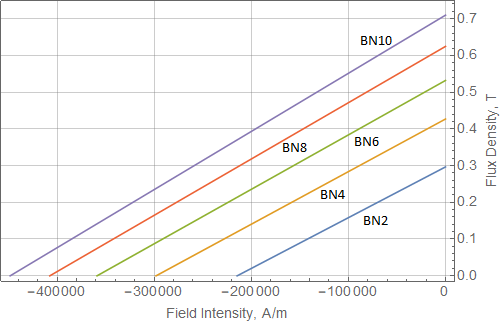
\includegraphics{bondedndfeb.png}
\caption{Representative 2nd quadrant demagnetization curves for FEMM's bonded NdFeB materials}
\end{figure}

\begin{table}
\centering
\begin{tabular}{|c|c|c|c|c|c|c|}
\hline
Grade & \(BH_{max}\), MGOe & \(B_r\), T & \(B_r\), kG & \(H_{cB}\), kA/m & \(H_{cB}\), kOe & \(\mu_r\)\\ \hline \hline
BN1 & 1 & 0.208 & 2.08 & 153 & 1.92 & 1.08\\ \hline
BN2 & 2 & 0.297 & 2.97 & 215 & 2.70 & 1.10\\ \hline
BN3 & 3 & 0.367 & 3.67 & 260 & 3.27 & 1.12\\ \hline
BN4 & 4 & 0.427 & 4.27 & 298 & 3.75 & 1.14\\ \hline
BN5 & 5 & 0.482 & 4.82 & 330 & 4.15 & 1.16\\ \hline
BN6 & 6 & 0.532 & 5.32 & 359 & 4.51 & 1.18\\ \hline
BN7 & 7 & 0.580 & 5.80 & 384 & 4.83 & 1.20\\ \hline
BN8 & 8 & 0.625 & 6.25 & 409 & 5.12 & 1.22\\ \hline
BN9 & 9 & 0.668 & 6.68 & 429 & 5.39 & 1.24\\ \hline
BN10 & 10 & 0.710 & 7.10 & 448 & 5.63 & 1.26\\ \hline
\end{tabular}
\caption{Representative Bonded NdFeB Material Grades at 20°C.}
\end{table}

\subsection*{References}
Bunting Magnetics Europe, \href{https://web.archive.org/web/20210307094900/https://e-magnetsuk.com/wp-content/uploads/2020/06/E-Magnets-UK-Bonded-Neodymium-Data-Sheet.pdf}{BREMAG Bonded NdFeB Standard Range}, accessed 03 Oct 2021.

\noindent Copyright 2026 David Meeker. This document is licensed under the \href{https://creativecommons.org/licenses/by/4.0/}{Creative Commons Attribution 4.0 International License (CC BY 4.0)}.

\end{document}
